\chapter{Introdução}\label{introducao}
Com o avanço dos computadores e das redes de comunicação, os sistemas de informação foram sendo transferidos dos computadores pessoais para os servidores \textit{web}, de onde eles podem ser acessados, virtualmente, a partir de todo o mundo. Para que esses sistemas funcionem, eles precisam de \textit{softwares} que atendam as requisições que chegam ao servidor a partir da rede de computadores usando o protocolo HTTP. Esses softwares são chamados Servidores HTTP.\\
Hoje o SIGA – Sistema Integrado de Gestão Acadêmica, desenvolvido utilizando a linguagem de programação PHP e o framework Miolo, utiliza o Apache HTTP \textit{Server} como servidor HTTP.\\

\section{Objetivos}
O objetivo desse estudo é identificar se a utilização do servidor HTTP Nginx é mais eficiente do que o utilizado atualmente, o Apache HTTP \textit{Server}.\\

\section{Objetivos Específicos}
Escrever!!!!!!

\section{Motivação}
Com a expansão das Universidades Federais, por ano são admitidos 3500 alunos na graduação, pós-graduação e graduação e especialização à distância, além de novos servidores técnicos-administrativos e professores. No final de 2.013, data do último levantamento, a Universidade Federal dos Vales do Jequitinhonha e Mucuri tinha 8.121 alunos, 576 professores e 421 servidores técnicos-administrativos, espalhados em quatro \textit{campi} universitários, fazendas experimentais e pólos de ensino em educação à distância, totalizando 9.118 pessoas que interagem com a universidade diariamente.\\
Em épocas de pico de utilização do SIGA, as reclamações de lentidão e problemas no sistemas são frequentes, as vezes impossibilitando a utilização do mesmo. Os picos mais notório são: fim de período letivo da graduação, quando alunos e professores acessam o sistema para olhar e lançar notas, respectivamente; e rematricula dos alunos da graduação, quando os mesmos escolhem as matérias que desejam cursar no período seguinte.\\
Com o crescente aumento de alunos, servidores públicos (professores e técnicos-administrativos) e teceirizados na universidade, a tendência é que a utilização do SIGA se torne mais problemática.
Com isso em mente, a utilização do servidor HTTP Nginx pode ajudar a amenizar os problema de desempenho do SIGA.\\

\subsection{Apache HTTP \textit{Server versus} Nginx}
O Apache, desde 1.995 tem sido o servidor HTTP mais utilizado no mundo. Em Outubro de 2.014, de acordo com pesquisa realizada em 1.028.932.208 de sítios pela empresa Netcraft, o Apache era usado por 37,79\% (385.354.994) desses sítios, com o Microsoft IIS aparecendo em segundo com 33,58\% (345.485.419) e o Nginx em terceiro com 14,42\% (148.330.190) de participação nos sítios.\\

\begin{figure}[h!]
	\centering
	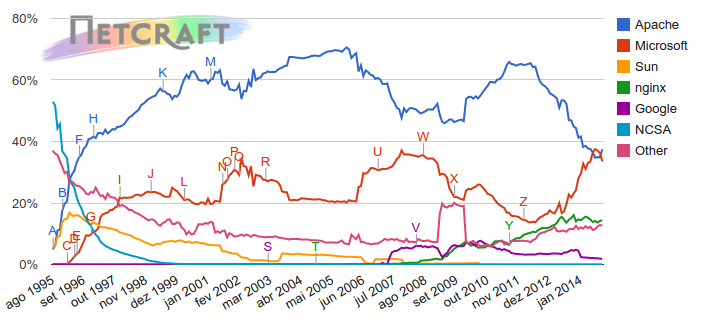
\includegraphics[width=0.6\linewidth]{figuras/grafico1}  
	\caption{Utilização de Servidores \textit{web} no mundo.}
	\label{fig:webservers-utilizacao}
\end{figure}

Nessa mesma pesquisa, entre os 1 milhão de sites mais acessados no mundo, o Apache é utilizado em 50,19\% (501,922), com o Nginx em segundo lugar com 14,36\% (25,588,943).\\

\begin{figure}[h!]
	\centering
	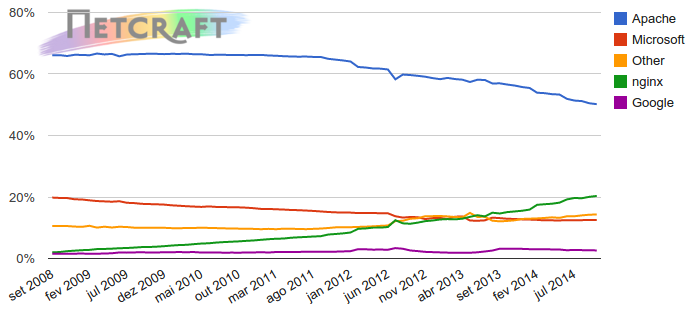
\includegraphics[width=0.6\linewidth]{figuras/grafico2} 
	\caption{Utilização de Servidores \textit{web} entre os 1.000.000 de sítios mais acessados no mundo.}
	\label{fig:webservers-utilizacao-milhao}
\end{figure}

Com a análise dos gráficos acima, é possível notar uma queda na utilização do Apache em detrimento de outros servidores HTTP, sendo mais notório a queda na utilização entre os 1 milhão de sítios mais acessados. É possível notar também o aumento no uso do Nginx, principalmente entre os 1 milhão de sítios mais acessados no mundo. É necessário frisar que só porque uma tecnologia está em ascensão significa que ela é melhor, mais é necessário investigar os motivos pelo qual tal tecnologia está crescendo em número de utilizadores.\\
Tendo sido desenvolvidos em épocas diferentes, o Apache e o Nginx tem formas diferentes de servir as requisições que chegam no servidor.\\
De acordo com \citeonline{rowe}, o Apache cria processos e \textit{threads} para lidar com as requisições. O administrador pode configurar o servidor para controlar o numero máximo de processos permitidos. Muitas \textit{threads} podem exaurir a memória principal(RAM) e pode forçar o servidor a usar memória \textit{SWAP}, degradando severamente o desempenho. Além disso, quando chega ao limite de processos, o Apache passa a recusar conexões.

\section{Organização do Trabalho}

